
% This LaTeX was auto-generated from MATLAB code.
% To make changes, update the MATLAB code and republish this document.

\documentclass{article}
\usepackage{graphicx}
\usepackage{color}

\sloppy
\definecolor{lightgray}{gray}{0.5}
\setlength{\parindent}{0pt}

\begin{document}

    
    
\subsection*{Contents}

\begin{itemize}
\setlength{\itemsep}{-1ex}
   \item Distributed Proportional Integral Observer
   \item PIO Test
\end{itemize}


\subsection*{Distributed Proportional Integral Observer}

\begin{par}
Sam Nazari March 2018
\end{par} \vspace{1em}
\begin{verbatim}
clear
clc

% Graph Structure
Ag = [0 1 1 1 0 0 0;
     1 0 1 1 1 0 0;
     1 1 0 0 0 1 0;
     1 1 0 0 0 0 1;
     0 1 0 0 0 0 1;
     0 0 1 0 0 0 1;
     0 0 0 1 1 1 0];

Deg = eye(7);
for i = 1:7
    Deg(i,i) = sum(Ag(i,:));
end

C = eye(7)

L = Deg-Ag

x0 = [0 1 1 0 0 0 0]

A = -L

% Condition: Distinct Eigenvalues
eig(A)

% Construct Fault Vectors
f1 = [1 0 0 0 0 0 0]'  % Vertex one is the intruder
f2 = [0 1 0 0 0 0 0]'  % Vertex two is the intruder
f3 = [0 0 1 0 0 0 0]'  % Vertex three is the intruder
f4 = [0 0 0 1 0 0 0]'  % Vertex four is the intruder
f5 = [0 0 0 0 1 0 0]'  % Vertex five is the intruder
f6 = [0 0 0 0 0 1 0]'  % Vertex six is the intruder
f7 = [0 0 0 0 0 0 1]'  % Vertex seven is the intruder

Ea = f2

% Choose the agent to be attacked
flt1  = 0;
flt2  = 1;
flt3  = 0;
flt4  = 0;
flt5  = 0;
flt6  = 0;
flt7  = 0;

% Choose a magnitude for the attack
f1Val = 10;
f2Val = 10;
f3Val = 10;
f4Val = 10;
f5Val = 10;
f6Val = 10;
f7Val = 10;

% Chose the attack time
tf1   = 2;
tf2   = 2;
tf3   = 2;
tf4   = 2;
tf5   = 2;
tf6   = 5;
tf7   = 7;

% Construct Disturbance Vectors
d1 = [1 0 0 0 0 0 0]'  % Vertex one undergoes a disturbance
d2 = [0 1 0 0 0 0 0]'  % Vertex two undergoes a disturbance
d3 = [0 0 1 0 0 0 0]'  % Vertex three undergoes a disturbance
d4 = [0 0 0 1 0 0 0]'  % Vertex four undergoes a disturbance
d5 = [0 0 0 0 1 0 0]'  % Vertex five undergoes a disturbance
d6 = [0 0 0 0 0 1 0]'  % Vertex six undergoes a disturbance
d7 = [0 0 0 0 0 0 1]'  % Vertex seven undergoes a disturbance

Ed = [d2,zeros(7,1) ,zeros(7,1)]

% Choose the agent to undergo a disturbance
dist1  = 0;
dist2  = 1;
dist3  = 0;
dist4  = 0;
dist5  = 0;
dist6  = 0;
dist7  = 0;

% Choose a magnitude for the disturbance
d1Val = 10;
d2Val = 10;
d3Val = 10;
d4Val = 10;
d5Val = 10;
d6Val = 10;
d7Val = 10;

% Chose the disturbance time
dt1   = 1;
dt2   = 1;
dt3   = 1;
dt4   = 1;
dt5   = 1;
dt6   = 4;
dt7   = 6;

% PIO 1

% This PIO is designed to be embedded in agent 1 in order to monitor faults
% in agents 2 and 3. This PIO monitors agent 2.

%bf1 = [0 1 0 0 0 0 0]'

% Observer matrices
c1 = [0 1 0 0 0 0 0;
      0 0 1 0 0 0 0;
      0 0 0 1 0 0 0]

% Make sure assumption 1 and 2 are met:
% Ass 1: rank(c1*Ed) = rank(Ed)
% Ass 2: for every re{lambda} > 0 rank(P) = dim(A) + dim(d) where P = [A-lam I Ed;C 0]

fprintf('rank(c1) = %i \n',rank(c1))
fprintf('rank(Ed) = %i \n',rank(Ed))
fprintf('rank(c1*Ed) = %i\n',rank(c1*Ed))

sys1 = ss(A,zeros(7,1),c1,0);
rank(obsv(sys1))
LP = place(A,c1',[-1,-2,-3,-4,-5,-6,-7])'
ALPC = A-LP*c1
LI = 10
ddot0 = 0;
xdot0 = zeros(7,1)';
TSIM = 10
sim('D_P_I_O')

% Plot errors
stateEstimErr = logsout.getElement(1)
distEstimErr  = logsout.getElement(2)
yhatEstimErr  = logsout.getElement(3)
figure
subplot(311)
title('State Estimation Error')
plot(stateEstimErr.Values,'LineWidth',2),grid on
subplot(312)
title('Disturbance Estimation Error')
plot(distEstimErr.Values,'LineWidth',2), grid on
subplot(313)
title('Output Estimation Error')
plot(yhatEstimErr.Values,'LineWidth',2), grid on

dhat.Name='Disturbance Estimate'
figure
title(dhat.Name)
plot(dhat, 'lineWidth',2),grid on
xlabel('Time (seconds)')
ylabel('Disturbance Estimate')
legend('Agent 2','Agent 3','Agent 4')
\end{verbatim}

        \color{lightgray} \begin{verbatim}
C =

     1     0     0     0     0     0     0
     0     1     0     0     0     0     0
     0     0     1     0     0     0     0
     0     0     0     1     0     0     0
     0     0     0     0     1     0     0
     0     0     0     0     0     1     0
     0     0     0     0     0     0     1


L =

     3    -1    -1    -1     0     0     0
    -1     4    -1    -1    -1     0     0
    -1    -1     3     0     0    -1     0
    -1    -1     0     3     0     0    -1
     0    -1     0     0     2     0    -1
     0     0    -1     0     0     2    -1
     0     0     0    -1    -1    -1     3


x0 =

     0     1     1     0     0     0     0


A =

    -3     1     1     1     0     0     0
     1    -4     1     1     1     0     0
     1     1    -3     0     0     1     0
     1     1     0    -3     0     0     1
     0     1     0     0    -2     0     1
     0     0     1     0     0    -2     1
     0     0     0     1     1     1    -3


ans =

   -5.4142
   -4.4142
   -4.4142
   -2.5858
   -1.5858
   -1.5858
   -0.0000


f1 =

     1
     0
     0
     0
     0
     0
     0


f2 =

     0
     1
     0
     0
     0
     0
     0


f3 =

     0
     0
     1
     0
     0
     0
     0


f4 =

     0
     0
     0
     1
     0
     0
     0


f5 =

     0
     0
     0
     0
     1
     0
     0


f6 =

     0
     0
     0
     0
     0
     1
     0


f7 =

     0
     0
     0
     0
     0
     0
     1


Ea =

     0
     1
     0
     0
     0
     0
     0


d1 =

     1
     0
     0
     0
     0
     0
     0


d2 =

     0
     1
     0
     0
     0
     0
     0


d3 =

     0
     0
     1
     0
     0
     0
     0


d4 =

     0
     0
     0
     1
     0
     0
     0


d5 =

     0
     0
     0
     0
     1
     0
     0


d6 =

     0
     0
     0
     0
     0
     1
     0


d7 =

     0
     0
     0
     0
     0
     0
     1


Ed =

     0     0     0
     1     0     0
     0     0     0
     0     0     0
     0     0     0
     0     0     0
     0     0     0


c1 =

     0     1     0     0     0     0     0
     0     0     1     0     0     0     0
     0     0     0     1     0     0     0

rank(c1) = 3 
rank(Ed) = 1 
rank(c1*Ed) = 1

ans =

     7


LP =

    1.4258    1.3753    0.5887
    2.6642    1.5090    0.1192
    1.5106    3.2990   -0.2920
    0.3865    0.0854    2.0368
    1.2235    0.1129   -0.1426
    0.1022    1.0379    0.0234
   -0.1241    0.0334    0.8533


ALPC =

   -3.0000   -0.4258   -0.3753    0.4113         0         0         0
    1.0000   -6.6642   -0.5090    0.8808    1.0000         0         0
    1.0000   -0.5106   -6.2990    0.2920         0    1.0000         0
    1.0000    0.6135   -0.0854   -5.0368         0         0    1.0000
         0   -0.2235   -0.1129    0.1426   -2.0000         0    1.0000
         0   -0.1022   -0.0379   -0.0234         0   -2.0000    1.0000
         0    0.1241   -0.0334    0.1467    1.0000    1.0000   -3.0000


LI =

    10


TSIM =

    10

Warning: Model 'D_P_I_O' is using a default value of 0.2 for maximum step size.
You can disable this diagnostic by setting Automatic solver parameter selection
to 'none' 

stateEstimErr = 

  Simulink.SimulationData.Signal
  Package: Simulink.SimulationData

  Properties:
              Name: 'stateEstimErr'
    PropagatedName: ''
         BlockPath: [1�1 Simulink.SimulationData.BlockPath]
          PortType: 'outport'
         PortIndex: 1
            Values: [1�1 timeseries]


distEstimErr = 

  Simulink.SimulationData.Signal
  Package: Simulink.SimulationData

  Properties:
              Name: 'distEstimErr'
    PropagatedName: ''
         BlockPath: [1�1 Simulink.SimulationData.BlockPath]
          PortType: 'outport'
         PortIndex: 1
            Values: [1�1 timeseries]


yhatEstimErr = 

  Simulink.SimulationData.Signal
  Package: Simulink.SimulationData

  Properties:
              Name: 'yhatEstimErr'
    PropagatedName: ''
         BlockPath: [1�1 Simulink.SimulationData.BlockPath]
          PortType: 'outport'
         PortIndex: 1
            Values: [1�1 timeseries]

  timeseries

  Common Properties:
            Name: 'Disturbance Estimate'
            Time: [63x1 double]
        TimeInfo: tsdata.timemetadata
            Data: [63x3 double]
        DataInfo: tsdata.datametadata

\end{verbatim} \color{black}
    
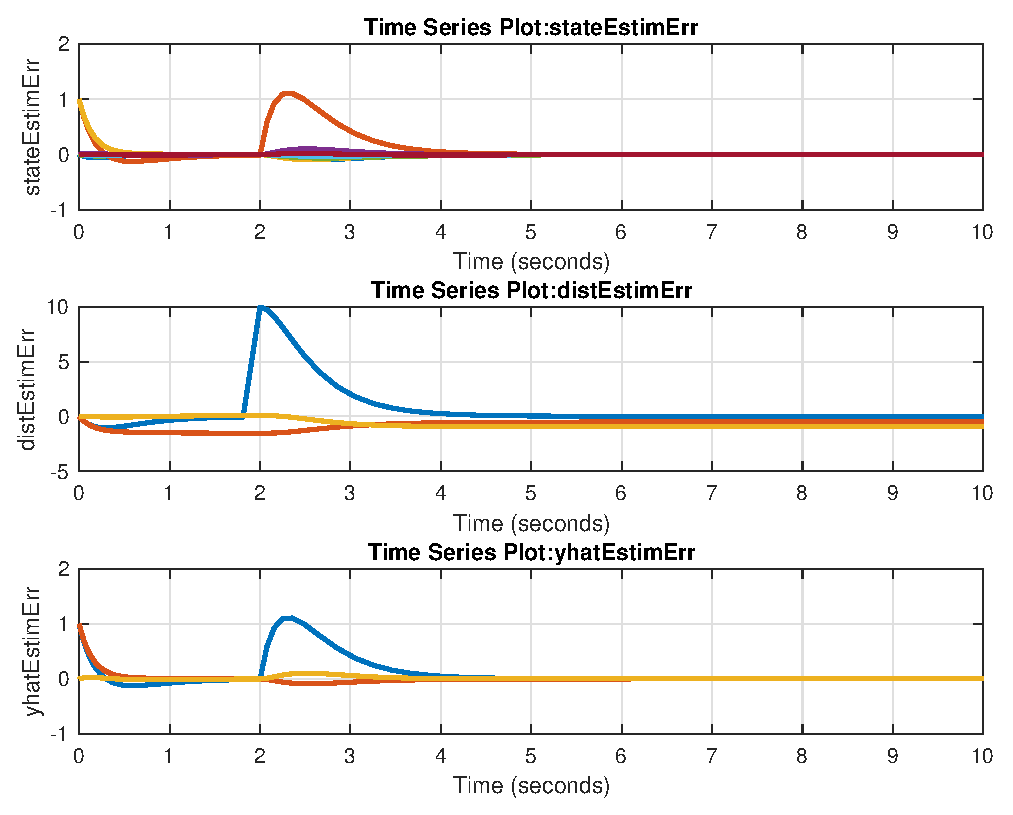
\includegraphics [width=4in]{D_PIO_01.eps}

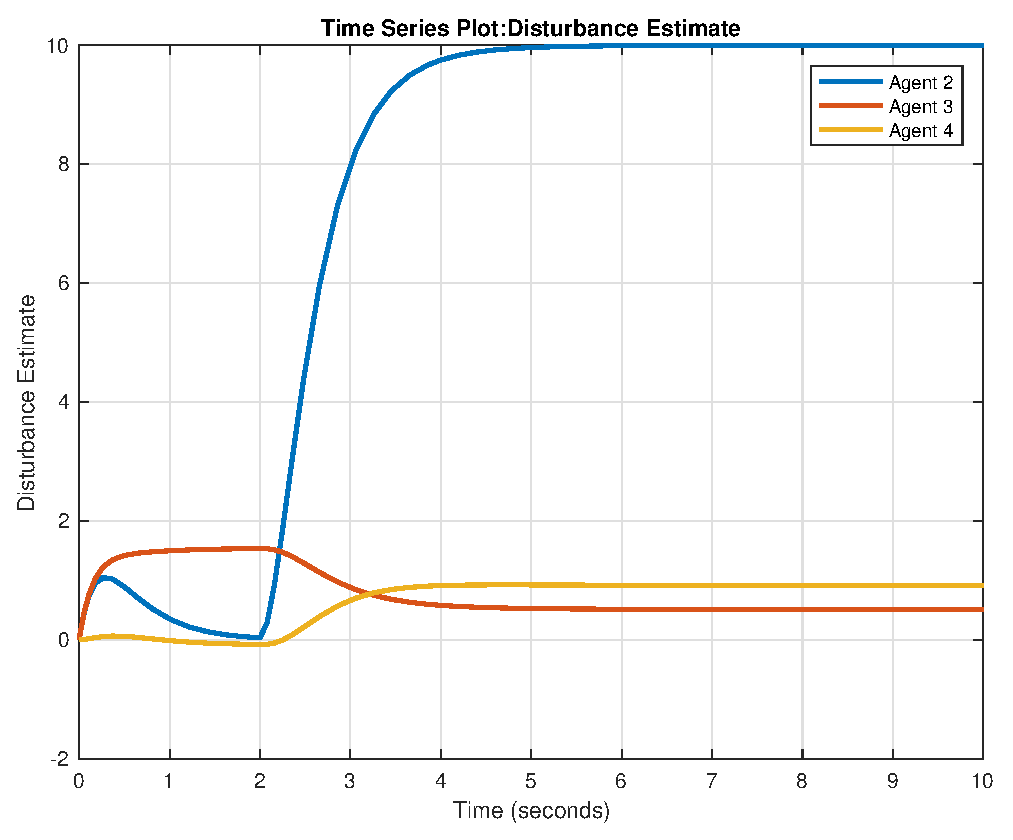
\includegraphics [width=4in]{D_PIO_02.eps}


\subsection*{PIO Test}

\begin{par}
A  = [-2 0;0 -3] B  = [1;-1] C  = eye(2) E  = [1;0] Ax = [A E;zeros(1,3)] Bx = [B;0] Cx = [C zeros(2,1)] sys= ss(Ax,Bx,Cx,0) rank(obsv(sys))
\end{par} \vspace{1em}
\begin{par}
warning off; cvx\_begin sdp variable P(3,3) variable G(3,2) minimize( 1 ) subject to P\ensuremath{>}=0; C1 = Ax'*P-Cx'*G'+P*Ax-G*Cx; C1\ensuremath{<}=0; cvx\_solver sedumi cvx\_end
\end{par} \vspace{1em}
\begin{par}
LI = place(A,C',[-1,-2]) LP = 10
\end{par} \vspace{1em}



\end{document}
    
